\documentclass[english,12pt,a4paper,final]{article}
\usepackage[T1]{fontenc}
\usepackage[left=2cm, right=2cm, top=2cm, bottom=2cm]{geometry}
\usepackage{amssymb,graphicx,amsfonts,amsthm, tikz, listings}
\usepackage{bookman}
\usepackage{babel}
\usetikzlibrary{shapes.geometric, arrows}
\begin{document}
	\begin{titlepage}
		\centering
		% TODO: \usepackage{graphicx} required
		
\includegraphics[width=0.15\textwidth]{logounesa.png}\par\vspace{1cm}
		{\Large \textsc{Assignment Report}\par}
		{\LARGE\bfseries Computational Mathematics\par}
		{\large \textsc{4420102183}\par}
		\vspace{7cm}
		Submitted by:\\[2ex]
		{\large\itshape Type your name}\\
		23030214XXX\\
		MA - 2023A
		\vfill
		Supervised by:\par
		Dimas Avian \textsc{Maulana}, M.Si.\\
		% Dr. Rahmawati Erma Standsyah, M.Si.\\ (untuk 2023B)
		
		\vfill
		{\large\textsc{Universitas Negeri Surabaya} \par}
		{\large\textsc{Faculty of Mathematics and Natural Sciences} \par}
		{\large\textsc{Bachelor of Mathematics} \par}
		\vspace{1cm}
		% Bottom of the page
		{\large \today\par}
	\end{titlepage}
	
	\section{Problem Statement}
	Describe the problem you solve today
	
	\section{\textit{Source Code}}
	Type the source code here. This is the example of source code:
	\lstinputlisting[language=python]{epidemiology.py} %ganti epidemiology.py dengan file Anda
	
	\section{Screenshots of Running Programme}
	\begin{figure}
		\centering
		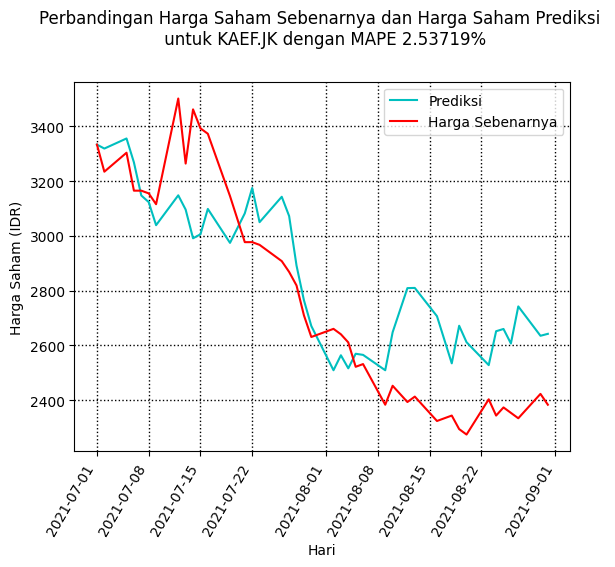
\includegraphics[width=\linewidth]{KAEF}
		\caption{Output of the programme with xxx}
		\label{fig:kaef}
	\end{figure}
	
	\section{Description}
	Give some descriptions on the problem you solve.
	
	\begin{thebibliography}{9} 
		\bibitem{Azuela} Mariano Azuela, \textit{The Underdogs: A Novel of the Mexican Revolution}, trans. Beth Jorgensen (New York: The Modern Library, 2002). 
	\end{thebibliography}
\end{document}